\chapter{超导磁体技术概论}
\section{引言}
超导磁体技术包括超导磁体的设计、制造和运行。为确保超导磁体成功、可靠、经济运行,需要提供最好的工程条件。
典型的10 T磁体要承受等效40 MPa的磁压,不论是以超导态运行于液氦(4.2 K)、液氮(77 K)还是以电阻态运行于室温。
超导磁体技术是一门交叉学科,需要包括机械、电气、制冷和材料在内的很多工程领域的知识和技能训练。

表\ref{first event}列举了与超导磁体技术有关的``首次"事件,特别是自1911年Onnes发现超导电性以来的重要事件。
关键的几个事件为:
\begin{enumerate}
  \item 水冷10 T电磁体:Francis Bitter,1930年代末
  \item 大规模氦气液化:Collins,1940年代末
  \item 磁体级超导体:Kunzler等,1960年代初
  \item 磁体低温稳定性:Stekly,1960年代中
  \item 高温超导体:Müller和Bednorz,1986年
\end{enumerate}

\begin{table}[htbp]\small
  \centering
  \caption{超导磁体技术有关的``首次"大事记} \label{first event}
\begin{threeparttable}
\begin{tabular}{ |c||l|}
\hline
时代 & 大事记\tnote{*}  \\ \hline
\multirow{4}{*}{1930s} & -Meissner效应 \\
 & -确认第II类低温超导体(LTS)\\
 & -超导电性的唯象理论 \\
 & -Bitter磁体产生高达10 T磁场 \\
 \hline
 1940s & -Collins氦气液化装置市场化\\
 \hline
\multirow{3}{*}{1950s} & -发现了更多的第II类超导体 \\
 & -超导电性的GLAG和BCS理论\\
 & -小型超导磁体 \\
 \hline
 \multirow{10}{*}{1960s} & -开发出磁体级超导体,即NbTi和$\mathrm{Nb_3Sn}$ \\
 & -国家磁体实验室建立\\
 & -Bitter磁体产生高达22 T(有铁芯时可达25 T)的磁场\\
 & -LTS中的磁通跳跃\\
 & -LTS/常规金属复合物超导体\\
 & -阐明低温稳定性标准\\
 & -大型冷却LTS磁体\\
 & -超导发电机\\
 & -内冷LTS磁体\\
 & -多丝NbTi/Cu超导体\\
 \hline
 \multirow{6}{*}{1970s} & -多丝$\mathrm{Nb_3Sn}$/Cu超导体 \\
 & -磁悬浮试验车\\
 & -加速器用超导双极和四极磁体 \\
 & -沟槽电缆导体(CICC)\\
 & -混合磁体产生30 T的磁场\\
 & -使用LTS磁体的NMR系统商业化\\
 \hline
  \multirow{5}{*}{1980s} & -使用LTS磁体的MRI系统商业化 \\
 & -聚变LTS磁体的多国协作试验项目(ITER,2001)\\
 & -60 Hz应用的亚微米超导体\\
 & -超导加速器\\
 & -发现高温超导体(HTS)\\
 \hline
   \multirow{4}{*}{1990s} & -BSCCO-2223/Ag超导带;磁体(1-7 T) \\
 & -``干式"磁体(LTS和HTS)\\
 & -YBCO涂层导体\\
 & -45 T混合磁体\\
 \hline
  \multirow{6}{*}{2000-} & -发现$\mathrm{MgB_2}$超导体,$T_c$=39K \\
 & -HTS示范装备,如电缆、变压器、电机\\
 & -高分辨率900 MHz-1 GHz全LTS NMR磁体 \\
 & -开发高分辨率LTS/HTS NMR磁体\\
 & -脑成像用高场MRI磁体\\
 & -强子对撞机(LHC)运行\\
 \hline
\end{tabular}
 \begin{tablenotes}
        \footnotesize
        \item[*] 各个时代的事件并非都如表中所列的顺序发生。缩写参见附录VI。%此处加入注释*信息
      \end{tablenotes}
    \end{threeparttable}
\end{table}

尽管Bitter的磁体是以水冷运行于室温的电阻型的,但我们可以放心的说,Bitter开创了现代磁体技术。
Collins液化设备出现后,曾经仅少数几个中心用得起的昂贵液氦实现广泛获取,快速推动了低温物理学的发展。
1950年代,很多重要的超导体被发现。到1960年代最终发展出一直使用到今天的磁体级超导体。

1960年代中期,Stekly等人提出的低温稳定磁体的设计准则或许可以称为超导磁体发展早期的最重要一步。
显然,它把超导从科学新奇引入到实际工程。
随后成功开发出的``高性能"(绝热,非低温稳定)磁体至今占据多数``市场"份额。

高温超导体的发现让超导磁体技术从液氦``高冷"中``热''起来。
伴随制冷技术的进步,高温超导体促进了用制冷机冷却的高温超导/低温超导干式磁体(无制冷剂)的发展。
21世纪以来,人们坚定的相信并热切的希望高温超导体最终能成功的实现低温超导体所未能实现的应用。

\section{超导电性}
超导电性的基本概念是在一特定``临界"温度($T_c$)下,在超导体内通过直流时,完全没有电阻。
除了临界温度$T_c$外,定义超导电性临界面的另两个参数是临界磁场($H_c$)和临界电流密度($J_c$)。
$T_c$和$H_c$是热力学参数,即对某一特定材料,不随金相处理过程而变;而$J_c$不是热力学参数。
实际上,Kunzler等人在1961年的关键贡献就是指出了对于某超导体,仅通过控制处理过程即可显著提高$J_c$。
本书不打算用形式化的唯象理论或微观理论来解释$T_c$、$H_c$、$J_c$间的相互关系。
不过,鉴于超导电性磁场下的行为在超导磁体中有重要作用,本书会用简单理论模型作扼要的解释。

\subsection{Meissner效应}
Meissner效应是由Meissner和Ochsenfeld在1934年发现的,描述的是在超导体内部磁感应强度$\vec{B}$不存在
(即$\vec{B}=0$)的现象。
超导体的完全抗磁性是比完全无电阻(即$\rho=0$)更根本的性质,因为材料的完全抗磁性
自动要求它是理想导体;反之则不然。
Meissner效应是产生于表面的超导电流,这在第I类和第II类超导体中都观察到了。
对第一类超导体,在其临界磁场$H_c$之下,Meissner效应都是存在的。而对第二类超导体,Meissner效应
仅存在于下磁场$H_{c1}$以下;外磁场超过$H_{c1}$后,会逐步进入超导体内,直到达到上磁场$H_{c2}$时完全进入。
此时,超导体成为完全的正常态。
%%迈斯纳效应图
\begin{figure}
  \centering
 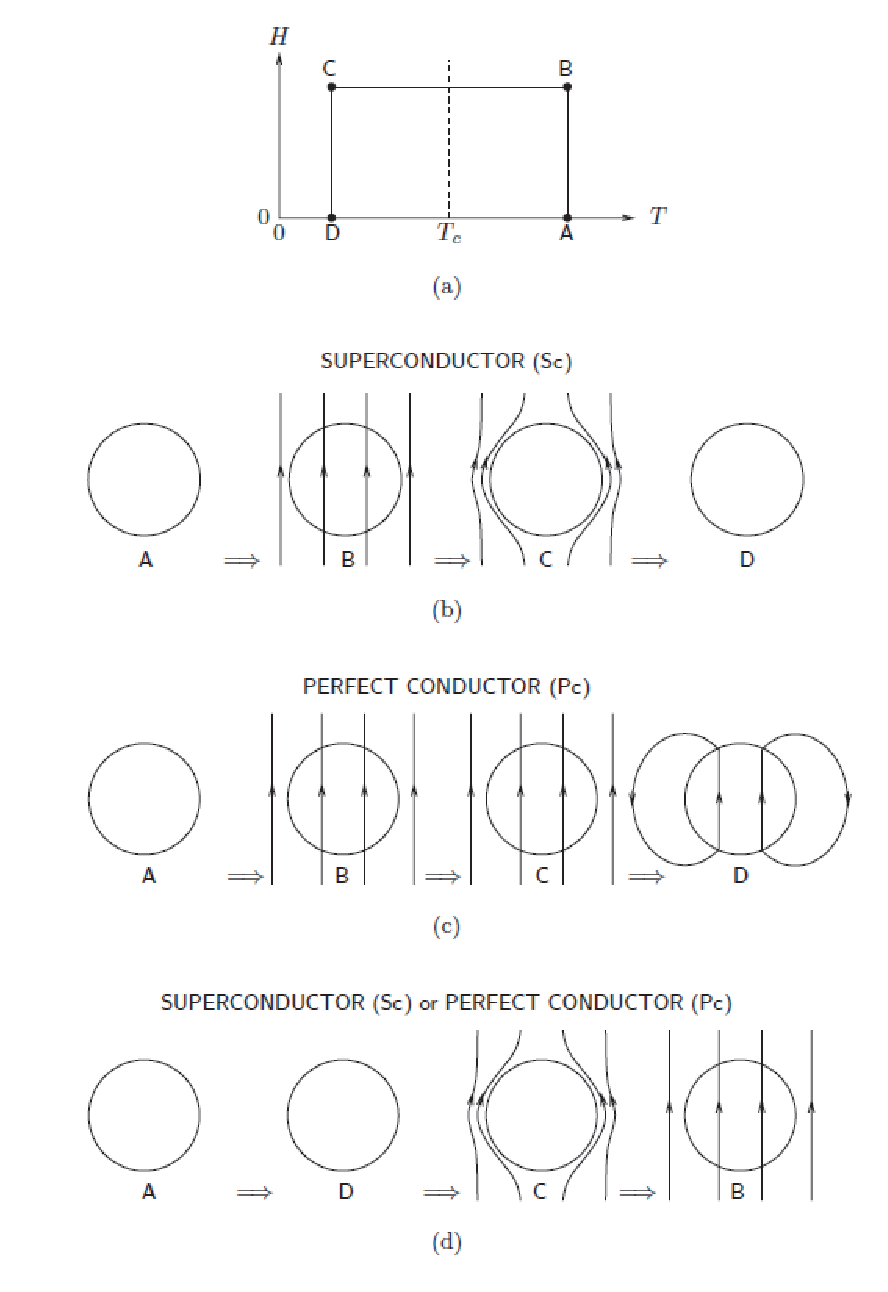
\includegraphics[scale=0.7]{chpt1/figs/fig1.1.eps}
  \caption{
(a): 两个球在$T <T_c$时的H-T相图,其中一个是超导体,另一个是理想导体。
(b): 超导球按$ A\rightarrow B\rightarrow C\rightarrow D$顺序施加H-T环境的磁场情况。
(c): 理想导体按相同的顺序施加H-T环境的磁场情况。
(d): 超导体或理想导体按$A\rightarrow D\rightarrow C\rightarrow B$顺序施加H-T环境的磁场情况。}
\end{figure}

\subsection{超导电性的London理论}
超导电性的唯象理论自1930年代开始发展(微观理论---BCS理论到1957年才完成)。其中,London电磁理论
(1935年)提出``穿透深度"概念来解释Meissner效应。简单的说,穿透深入为$\lambda$的表面超导电流
完全屏蔽了超导体外磁场。根据London理论,$\lambda$由下式给出:
\begin{equation}
\lambda=\sqrt{\frac{m}{\mu_0 e^2 n_{se}}}
\end{equation}
式中,$m$和$e$分别是电子质量($9.11\times 10^{-31}\ \mathrm{kg}$)和电荷量($1.60\times 10^{-19}\ \mathrm{C}$);$\mu_0$是自由空间磁导率($4\pi \times 10^{-7}\ \mathrm{H/m}$)。
这里,超导电子密度$n_{se}$与自由电子$n_{fe}$不同:在$T=0$时,所有电子都是超导电子;在$T=T_c$时,无超导电子。定量地,有:
\begin{equation}
n_{se}\approx n_{fe}=\frac{\rho N_A}{W_A}
\end{equation}
其中,$\rho$是导体的密度($\mathrm{g/cm^3}$),$N_A$是Avogadro常数($6.023\times 10^{23}/\mathrm{mole}$),$W_A$是
原子质量($\mathrm{g/mole}$)。超导电流密度$J_c=e n_{se} v\approx e n_{fe} v$,$v$是超导电子的漂移速度。

\subsection{第I类和第II类超导体}
1911年,Onnes在纯汞中发现了超导电性;随后,铅、锡等其他金属也被发现是超导体。
这些材料,被称为第I类超导体。第I类超导体$H_c$较小(0.1 T),并不适合做超导磁体的材料。
磁体级超导体属第II类,是由Haas和Voogd于1930年首先在铅铋合金中发现。

第II类超导体可以用第I类超导体和正常导体材料的混合态来建模。
1960年代初,有两种混合态物理模型:薄层模型(lamina)和岛模型(island)。
薄层模型是Goodman提出的,他认为第II类超导体的超导态层被正常态层分割开。
岛模型是Abrikosov提出的,不久得到了Essmann和Trauble的实验证实。
该理论认为在超导``海"中存在许多正常态的``岛"。对于第II类超导体,若要在0. 1T以上还能保持超导态,
正常态``岛"的半径必须小于$\lambda$。岛半径是空间参数---相干长度$\xi$,该参数是Pippard在1953年引入的。

$\xi$定义了超导/正常态转变发生的距离。根据用于解释第II类超导体磁场性质的GLAG理论,
如果某超导体的$\xi < \sqrt{2}\lambda$,则属于第II类;$\xi >\sqrt{2}\lambda$,则属于第I类。
合金中由于自由电子的平均自由程缩短,$\xi$减小。
$\xi$反比于材料正常态的电阻率。两种常用的磁体级超导体---$\mathrm{NbTi}$和$\mathrm{Nb_3Sn}$
---的室温正常态电阻率都比铜打出一个数量级。值得注意的是,所有HTS的$\xi$都远小于$\lambda$。

\begin{figure}[htbp]
	\centering
	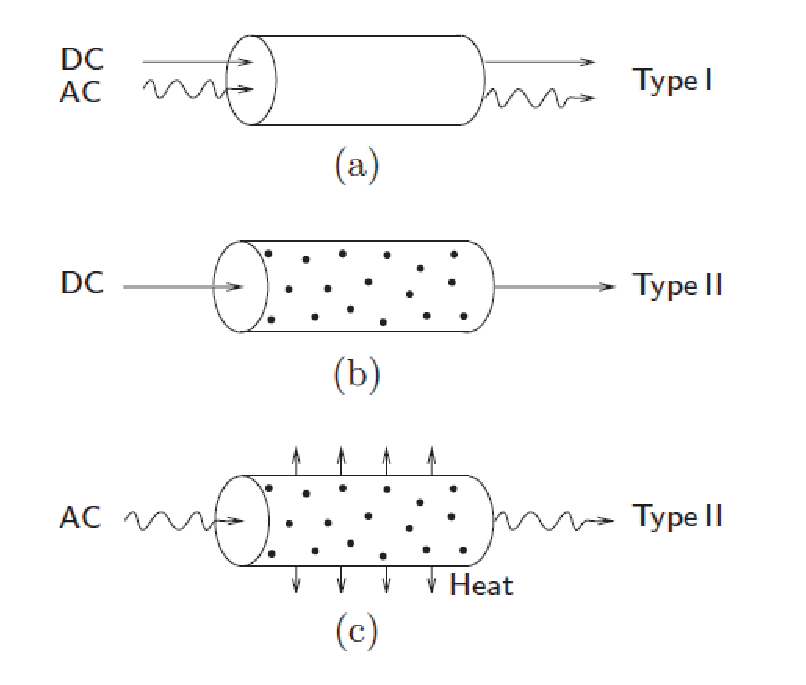
\includegraphics[scale=0.6]{chpt1/figs/fig1.2.eps}
	\caption{
		载流超导棒。 (a) 第I类超导体棒, DC或AC---无焦耳耗散产生;
		(b) 第II类超导体棒,DC无耗散;(c) 第II类超导体棒,AC有焦耳热耗散产生。}\label{acdccurrent}
\end{figure}

\subsubsection{DC和AC响应}
图~\ref{acdccurrent}给出了三根超导棒的示意图。
第I类棒(1.2a)和第II类棒(1.2b,1.2c)中的载流均小于其临界电流。
在第I类超导体中,无论通过AC抑或DC,电流都只在表面(London穿透深度)流过且无能量耗散。
第II类超导体中,DC在整个棒体内流过,尽管存在正常区,但不产生耗散。
我们可以想象为``超导电子"通过材料时``躲"开了正常态区域。
从电路的观点看,可以认为这些有电阻的``岛"被周围的超导``海"短路掉了。
当通以AC时,第II类超导体是有损耗的,即存在电阻---尽管其有效电阻仍然比正常高导电金属小几个数量级。
每一个正常态区域都包含磁通束,称为磁通量子(fluxoid)或旋涡(vortices)。
磁通束在时变磁场和/或电流下``流"动。此种耗散性磁通流动是第II类超导体交流损耗的主要来源。

\subsubsection{磁场性质}
第I类超导体在$H<H_c$下是完全抗磁的;超过$H_c$后就成为常规的无磁材料。
第II类超导体在$H_{c1}$下,磁场性质和第I类一样;在$H_{c1}$和$H_{c2}$之间时,第II类超导体是混合态。
图~\ref{mhcurve}给出了第I类/第II类超导体的磁化强度与磁场强度的关系。
注意,磁体级超导体的磁化曲线都是不可逆的,并非如图中一样。不可逆的结果之一就是存在磁滞。
第II类超导体的磁滞本性是其交流损耗的又一来源。

%%磁化曲线
\begin{figure}[htbp]
  \centering
 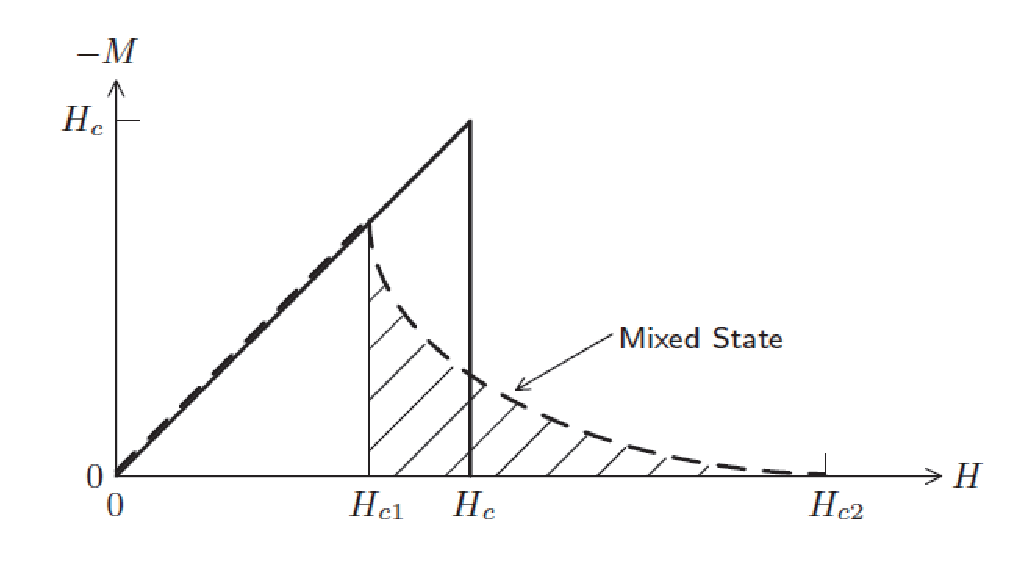
\includegraphics[scale=0.6]{chpt1/figs/fig1.3.eps}
  \caption{
超导体的M-H关系。实线是第I类,虚线是第II类。斜线填充区域表示第II类超导体的混合态。
}\label{mhcurve}
\end{figure}

\subsubsection{超导体举例}
表~\ref{criticalparameters}列出了一些超导体,并给出了其类型、零场临界温度$T_c$、临界磁感应强度
(第I类为$\mu_0H_c$;第II类为$\mu_0H_{c2}$)。所有的金属都是第I类超导体,临界场很小。
这就解释了为什么Onnes在1913年试图用铅线做超导磁体会失败:在很小磁场下,铅就失超了。
即使Onnes时代,磁场也要达到0.3 T才有使用价值。表\ref{criticalparameters}已经很清楚的表明,
超导磁体必须使用第II类超导体。
和第I类超导体不同,第II类超导体存在多种类型:合金、金属混合物甚至氧化物。
所有的高温超导体都是氧化物。$\mathrm{MgB_2}$非金属,也被归为高温超导体。
图~\ref{tcvsyear}给出了几种代表性的HTS或LTS的$T_c$及其发现年份。
图中还标出了重要制冷工质的沸点。
其中,实线把氧化物超导体连缀了起来,虚线把金属超导体连缀了起来。

\begin{table}[htbp]\small%%表1.2
  \centering
  \caption{几种代表性第I类和第II类超导体的临界温度和临界磁场} \label{criticalparameters}
\begin{threeparttable}
  \begin{tabular}{|l|c|c||l|c|c|}
    \hline
    % after \\: \hline or \cline{col1-col2} \cline{col3-col4} ...
    第I类 & $T_c$[K] & $\mu_0 H_c$\tnote{*}[T] & 第II类 & $T_c$[K] & $\mu_o H_{c2}$\tnote{*}[T] \\ \hline 
    Ti & 0.39 & 0.0100 & Nb & 9.5 & 0.2\tnote{*} \\ \hline
    Zr & 0.55 & 0.0047 & NbTi & 9.8 & 10.5\tnote{$\dagger$} \\ \hline
    Zn & 0.85 & 0.0054 &NbN & 16.8 & 15.3\tnote{$\dagger$} \\ \hline
    Al & 1.18 & 0.0105&$\mathrm{MgB_2}$ & 39.0 & 35-60\tnote{$\ddagger$}\\ \hline
    In & 3.41 & 0.0281 & $\mathrm{Nb_3Sn}$ & 18.2 & 24.5\tnote{$\dagger$}  \\ \hline
    Sn & 3.72 & 0.0305  & $\mathrm{Nb_3Al}$ & 18.7 & 31\tnote{$\dagger$}\\ \hline
    Hg & 4.15 & 0.0411  & $\mathrm{Nb_Ge}$ & 23.2 & 35.0\tnote{$\dagger$}\\ \hline
    V & 5.38 & 0.1403& YBCO & 93 & 150\tnote{*}\\ \hline
    Pb & 7.19 & 0.0803 & $\mathrm{Bi_2Sr_2Ca_{n-1}Cu_{n}O_{2n+4}}$\tnote{$\star$} & 85-110 & >100\tnote{*} \\
    \hline
  \end{tabular}
 \begin{tablenotes}
        \footnotesize
        \item[*] 0 K, 估计值。 %此处加入注释*信息
        \item[$\dagger$] 4.2 K, 估计值。%此处加入注释**信息
        \item[$\ddagger$] 4.2 K, 估计值(35 T,平行场,60 T,垂直场)。%此处加入注释**信息
        \item[$\star$] $n=2$, Bi2212; $n=3$, Bi2223。%此处加入注释**信息
      \end{tablenotes}
    \end{threeparttable}
\end{table}


\begin{figure}%%图1.4
  \centering
 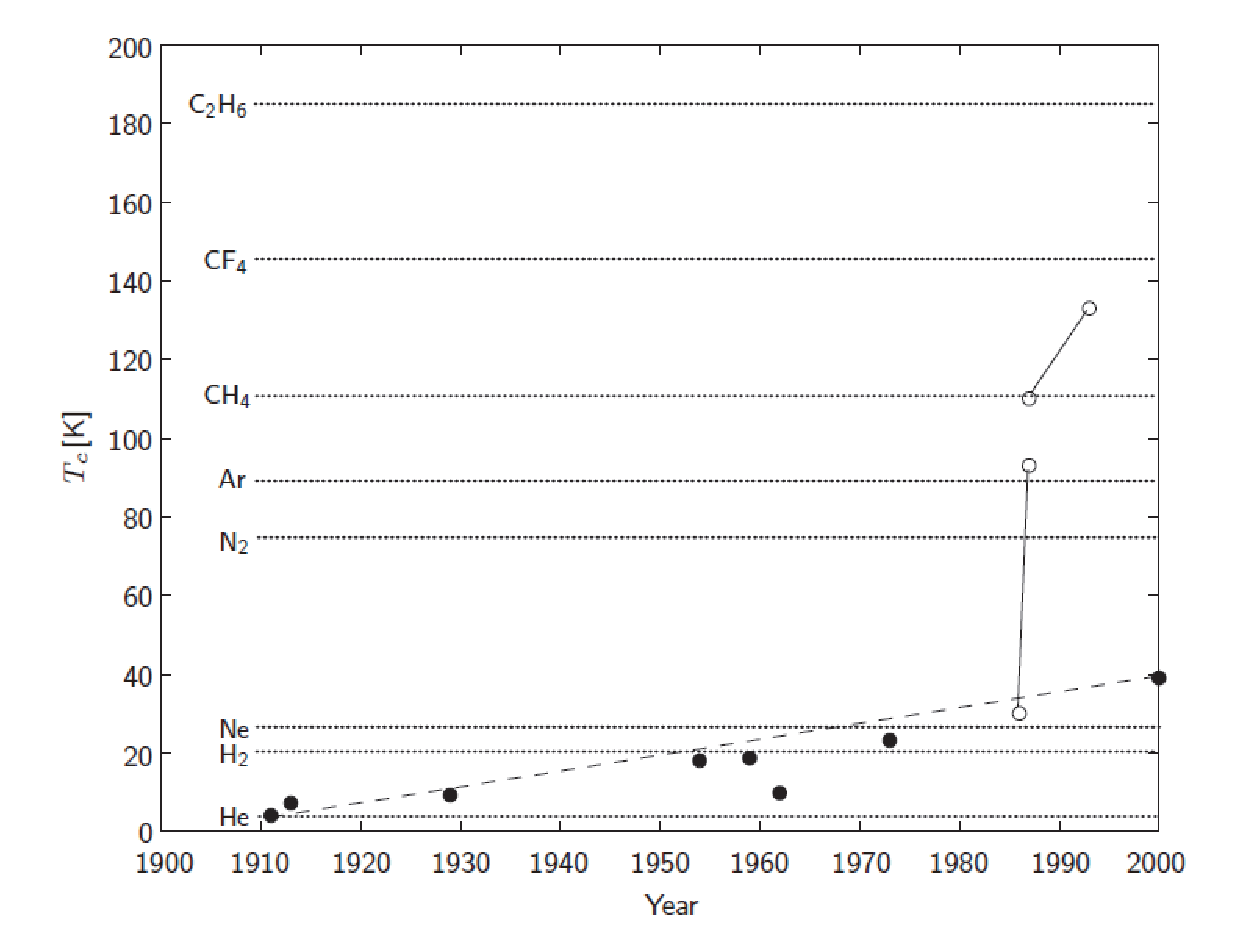
\includegraphics[scale=0.6]{chpt1/figs/fig1.4.eps}
  \caption{
几种代表性超导体$T_c$和发现年份。实线和空心圆圈:HTS;虚线和实心圆圈:LTS(2000年发现的$MgB_2$除外,
其$	T_c$=39 K,被认为是HTS)。水平点线:若干制冷剂的沸点温度,自下而上分别为:
He(4.22 K);$\mathrm{H_2}$(20.39 K);Ne(77.36 K);$\mathrm{N_2}$(77.36 K);Ar(87.28 K);
$\mathrm{CH_4}$(111.6 K);$\mathrm{CF_4}$(145.4 K);$\mathrm{C_2H_6}$(184.6 K)。
}
\end{figure}


\subsection{第II类超导体的临界面}
图1.5给出了一种典型的第II类磁体级超导体的临界面。超导电性存在于由边界函数$f_1,f_2,f_3$所确定的临界面之下。对磁体工程师更有用的是通用的$f(H,T,J)$函数。
\begin{figure}
  \centering
 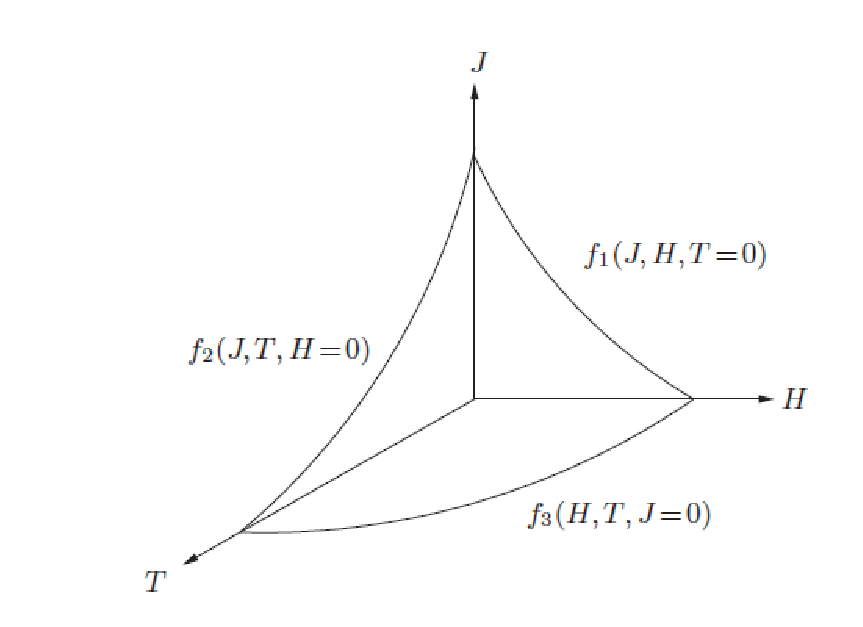
\includegraphics[scale=0.6]{chpt1/figs/fig1.5.eps}
  \caption{
典型第II类超导体的临界面
}\label{ciriticalsurface}
\end{figure}

\subsubsection{临界电流密度,$J_c$}
第II类超导体的$J_c$可以通过金相处理的方式大大提高。这种增强的$J_c$性能通常归因于产生的``钉扎中心"钉住了旋涡,
从而可以抵抗施于其上的Lorentz力($\vec{J}_c\times \vec{B}$)。
钉扎中心可通过材料掺杂、金相处理(如冷处理产生错位,热处理产生前位体和晶界)等手段产生。Kim等给出:
\begin{equation}
  J_c\approx \frac{\alpha_c}{H+H_0}\
\end{equation}
式中,$\alpha_c, H_0$是常数。$\alpha_c$是$H\gg H_0$时与Lorentz力密度平衡的渐近力密度。

\section{磁体级超导体}
磁体级超导体是指那些满足严格的磁体参数要求且可商业化获取的超导体。
以下是对磁体级超导体和超导材料的简明讨论简短评论:现今每一种成功的磁体级超导体,
都经历了长期和复杂的发展过程才从实验室走出。

\begin{table}[htbp]\small
  \centering
  \caption{超导材料 vs. 磁体级超导体} \label{scmaterialvsconductor}
\begin{tabular}{|l|c|l|c|}
  \hline
  标准 & 数量 & 标准 & 数量 \\ \hline
  1. 能超导? & ~10000 & 3. $J_c>1\ \mathrm{GA/m^2}$? & ~10 \\ \hline
  2. $T_c> 4.2\ \mathrm{K}$且$\mu_0 H_{c2}>10\ \mathrm{T}$? &~100 & 磁体级? & <10 \\
  \hline
\end{tabular}
\end{table}

\subsection{超导材料 vs. 磁体级超导体}
表\ref{scmaterialvsconductor}给出了满足特定标准的材料数量。可见,随着标准推向磁体级,数量急剧减少。
实际上,当今发现的10000多种超导体中,仅有几种可用于超导磁体。它们包括低温超导体NbTi、$\mathrm{Nb_3Sn}$;
高温超导体Bi-2212、Bi-2223、YBCO以及$\mathrm{MgB_2}$。

\subsection{实验室级超导体 vs. 磁体级超导体}
超导材料从实验室级到磁体级要经过很长的一段历程。可分为六个阶段:
\begin{enumerate}
  \item 发现;
  \item 提高$J_c$性能
  \item 与基底金属的共处理;
  \item 多丝成形;
  \item $I_c>100\ \mathrm{A}$且长度$>1000\ \mathrm{m}$;
  \item 其他要求,如强度和应力容许值。
\end{enumerate}

表\ref{scstage}给出了$\mathrm{Nb_3Sn}$和Bi-2223的上述六个阶段开始的大致时间。
Bi-2223最开始是与常规金属银共处理的,其阶段2一直持续到今天。
对于涂层YBCO,目前大致处于阶段3晚期,即将进入阶段4。
目前已有使用YBCO制作的运行于77 K的小线圈。
2001年发现的$\mathrm{MgB_2}$已进入阶段5,目前已有``大"$\mathrm{MgB_2}$磁体建成投运。

1961年发现的$\mathrm{Nb_3Sn}$经过十多年紧张的R\&D后,到目前在多数磁体应用时,仍需由用户定制材料性质。
$\mathrm{Nb_3Sn}$的脆性及其承受应力不能超过$~0.3\%$的约束本质上决定了它是不易处理的,
需要十分小心谨慎;BSCCO与此情形很类似。

\begin{table}[htbp]\small
  \centering
  \caption{$\mathrm{Nb_3Sn}$和Bi-2223从材料到导体的发展阶段} \label{scstage}
\begin{tabular}{|c|l|l|l|}
  \hline
  阶段&事件& $\mathrm{Nb_3Sn}$ &Bi-2223 \\ \hline
1 & 发现 & 1950年代早期& 1980年代晚期 \\ \hline
2 & 做成大$J_c$短样 & 1960年代早期 & 1990年代早期\\ \hline
3 &与基底金属共处理&1960年代晚期&1990年代早期\\ \hline
4 &多丝成形&1970年代早期&1990年代中期\\ \hline
5 &$I_c\ge 100\ \mathrm{A}$;长度$\ge 1000\ \mathrm{m}$ &1970年代中期&2000年代早期\\ \hline
6 &其他磁体需求&1970年代晚期&2000年代中期\\
  \hline
\end{tabular}
\end{table}


\section{磁体设计}
\subsection{要求和关键点}
磁体无论直接用于实验还是作为大系统的一个组件,都必须满足磁场的基本要求:规定的空间分布和规定时变特性。
磁场的特性常由以下重要参数给定:1. $H_0$,磁体中心($x=0, y=0, z=0$)场强;
2. $V_0$,规定磁场的空间区域;
3. $H(t)$,磁场的时变特性。其中,特征1和3,在第二章和第三章中有详细讨论。
除了满足以上基本要求,磁体设计还必须满足以下几个关键点:
\begin{description}
  \item[机械完整性] 磁体必须有足够的结构强度,承受正常运行和故障时的巨大磁场应力。
  \item[运行可靠性] 磁体必须能稳定、可靠的达到并持续工作于运行点。
  磁体的这种稳定性,一般简称为磁体稳定性。运行中磁体失去超导电性的过程叫\textbf{``失超"}。
  \item[保护] 一旦发生可能导致磁体变成正常态的事件,必须能保证其不被损坏并且能在事件解除后可再次励磁并
  工作于运行点。
  \item[导体] 对量产的磁体,超导磁体系统的费用很大程度上受超导体费用的影响,即导体费用决定磁体费用。
  本书定量处理少数几个有关多种方案经济性选择的导体费用问题,比如
NbTi@1.8 K,$\mathrm{Nb_3Sn}$@4.2 K,NbTi@4.2 K,$\mathrm{MgB_2}$@15 K。
  \item[制冷] 磁体运行需要能量来创造并维持低温环境,故制冷是超导磁体的一个重要问题。
  人们常过分强调制冷对于整个系统的重要性。故这里必须指出,哪怕在超导磁体是作为关键部件的很多应用中,
  磁体也不过是整个系统的一个组件,而制冷则又是磁体的一个组件。
  制冷系统的功耗通常仅占整个系统的一个很小分数。
\end{description}

磁体的终极发展目标是市场化。若想取得市场成功,还需要考虑两点:1. 价格;2. 易用性。

\subsection{运行温度的影响}
LTS磁体的基本温度通常是4.2 K;仅HTS磁体的运行温度可能高于4.2 K。
运行温度会影响到磁体的五个方面:机械完整性、稳定性、保护、导体和制冷。
图1.6给出了``难度或费用"与运行温度的定性关系。
%图1.6
\begin{figure}
  \centering
 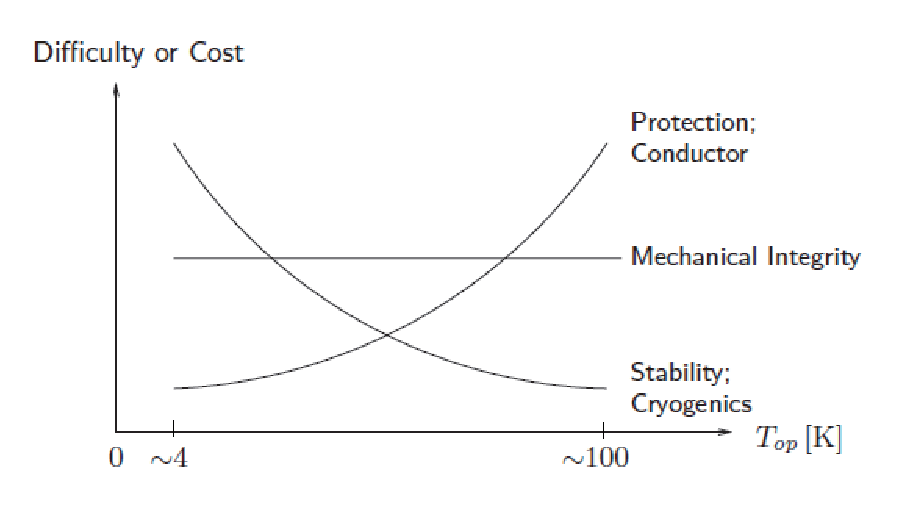
\includegraphics[scale=0.6]{chpt1/figs/fig1.6.eps}
  \caption{
温度对磁体的五个关键点的影响
}\label{temperatureeffect}
\end{figure}

通常,LTS的运行温区是1.8-10 K,HTS是20-80 K。LTS/HTS混合系统,运行温度由LTS决定,一般<10 K。
图\ref{temperatureeffect}~中,保护与导体、稳定性与制冷用同一条曲线,仅表示趋势,并不代表实际上的重合。

图\ref{temperatureeffect}~表明,机械完整性的要求基本与运行温度无关。这个结论在运行温度到100 K之间都是适用的。
在这个温区内,磁体的不同材料的热膨胀都可忽略。
对给定磁场要求的磁体,安匝数与运行温度基本无关。因为已知的超导体的临界电流密度都是随温度上升而下降,
而导体费用总是随温度上升而提高:降低制冷费用的期望收益一定要与导体费用的增加值作比较。
运行稳定性和保护受运行温度影响较大。

\section{数值解}
本书开篇已指出,超导磁体技术是一门交叉学科,需要精湛的机械、电气、制冷和材料领域的专业知识。
其实这也意味着一个人是不可能完成满足每一个实际磁体设计和运行参数需求的可靠的数值解的。
通常,需要一个专业的团队来做成此事。
\subsection{粗算解}
制冷工程师或其他成员没必要对磁场专家的所有计算深信不疑,制冷专家也应当能够计算比较复杂条件下的大致磁场。
本书的一个目标就是让设计团队的每一个成员都具备在自己领域以及其他领域进行估算的能力。
实际上,每一个新磁体系统的研发都应以此开始:每一个成员都来对每一个重要的设计和运行参数粗算一遍;
而后,由组内领域专家完成磁体制造和运行的更精确的数值计算。

\subsection{程序解}
磁体系统的实际制造和运行的每一个设计和运行参数一般都必须采用程序辅助计算。
多数设计团队使用ANSYS、VectorFields、COMSOL,这几种软件都可用于磁场、应力应变以及热的分析。
GANDALF、THEA等专用程序专门用于处理CICC导体绕制的大型磁体(特别是聚变磁体)的失超产生和传播现象。
失超现象包含的热、流体、电暂态、电缆和工质等的变化很大,热、电物性的变动幅度常跨越1-2个数量级。
正是这个原因,失超暂态多(有时完全是)依赖于数值仿真。数值仿真能处理非线性的热能产生和传导以及工质因受热引起的可压缩黏性流动。
上述每一套程序都凝结了大量专家超过25年的大量工作。

GANDALF和THEA都是商业软件。GANDALF最初是用来分析ITER导体的热-流体暂态的。THEA的主要特征是将热、流体模型扩展到多平行通道。
%【此句不通】如多丝具有不同温度,平行流通道,包括非均一电流分布和暂态重分配。

\section{专题}
\subsection{问题1.1:第I类超导体的热力学性质}
第I类超导体的单位体积比热($\mathrm{J/m^2K}$)由下式给出:
\begin{subequations}\label{eqn:1.4ab}
	\begin{align}
\mbox{超导态:} C_s(T) &= aT^3 \\
\mbox{正常态:} C_n(T)&= bT^3+\gamma T	
	\end{align}
\end{subequations}
式中,$a,b,\gamma$都是常数。

a) 证明零场时的临界温度为:
\begin{equation}\label{eqn:1.5}
  T_c=\sqrt{\frac{3\gamma}{a-b}}
\end{equation}
提示:1) 熵的表达式$C(T)=T\frac{\partial S(T)}{\partial T}$;2) $H=0$时,有$S_n(T_c)-S_s(T_c)=0$。

b) 证明$H_{c0}$在$T$=0 K,$H_{c0}\equiv H_c(0)$时,可由下式给出:
\begin{equation}\label{eqn:1.6}
  H_{c0}=T_c \sqrt{\frac{\gamma}{2\mu_0}}
\end{equation}

证明临界磁场$H_c(T)$是$T$的二次函数:
\begin{equation}\label{eqn:1.7}
  H_c(T)=H_{c0}\left[1-\left(\frac{T}{T_c}\right)^2\right]
\end{equation}
提示:零场时单位体积的吉布斯自由能关系为:
\begin{equation}\label{eqn:1.8}
  G_n(T)-G_s(T)=\frac{1}{2}\mu_0 H_c^2(T)
\end{equation}
根据1.8式以及$S(T)=-\partial G(T)/\partial T$,可以推导出1.6式。

c) 证明内能密度差$U_n-U_s$在自场下于$T_{ux}$时取最大:
\begin{equation}
  T_{ux}=\frac{T_c}{\sqrt{3}}
\end{equation}
提示:在零场时有$U(T)=\int C(T)dT$。

d) 缓慢绝热地向超导磁体施加磁场(初始温度为$T_i$,$0<T_i<T_c$)至略大于其临界值,
此时超导体相变为正常态。降低导体温度到$T_j (<T_i)$,给出$T_i$和$T_j$的关系,并
画出本过程的热力学相图。

e) 同样对d)中的超导体,初始温度为$T_i$($0<T_i<T_c$),置于零场中,突然施加$H_e$。
如果$H_e$超过临界值$H_{ec}$,材料将被加热。证明
\begin{equation}
  H_{ec}(T_i)=H_c(T _i)\sqrt{\frac{1+3(T_i/T_c)^2}{1-(T_i/T_c)^2}}
\end{equation}

\subsubsection{问题1.1之解答}
a) 由于$C(T)=T\frac{\partial S(T)}{\partial T}$以及$S(T=0)=0$,我们有
\begin{align*}
S(T) =\int_{0}^{T}C(T)dT \tag{S1.1} 
\end{align*} 

将1.4式代入,有:
\begin{align*}
S_s(T) =\int_{0}^{T}\frac{C_s(T)}{T}dT=\frac{1}{3}aT^3 \tag{S1.2a}
\end{align*} 
\begin{align*}
S_n(T) =\int_{0}^{T}\frac{C_n(T)}{T}dT = \frac{1}{3}bT^3 + \gamma T \tag{S1.2b}
\end{align*} 

于是,
\begin{align*}
S_n(T) − S_s(T) =\gamma T − \frac{1}{3} (a − b)T^3\tag{S1.3}
\end{align*} 

上文已指出,在$H=0$时,有$S_n(T_c)−S_s(T_c)=0$,所以
\begin{align*}
\gamma= \frac{1}{3} (a − b)T^2 \tag{S1.4}
\end{align*}

解出$T_c$,有
\begin{align*}
T_c=\sqrt{\frac{3\gamma}{a-b}} \tag{1.5}
\end{align*}

b) 从式1.8以及$S(T)=−\partial G(T)/\partial T$,有
\begin{align*}
S_n(T) − S_s(T) = −\mu_0 H_c(T)\frac{\partial H_c(T)}{\partial T}\tag{S1.5}
\end{align*}

联立S1.3和S1.4,并利用$(a-b)/3=\gamma/T_c^2$,有
\begin{align*}
S_n(T) − S_s(T)=\gamma T\left[1-\left(\frac{T}{T_c}\right)^2\right]  \tag{S1.6}
\end{align*}

联立上面两式,对$T$积分,有
\begin{align*}
−\frac{1}{2}\mu_0 H_c^2(T) =\frac{1}{2}\gamma T_c^2-
\frac{1}{4}\gamma T_c^2 \left(\frac{T}{T_c}\right)^4+A \tag{S1.7}
\end{align*}
式中,$A$是常数。由于$H_c(T =0)\equiv H_{c_0}$,我们有$A=−\mu_0 H_{c_0}^2 / 2$。在
$T=T_c$时,由于$H_c(T_c)=0$,上式成为
\begin{align*}
0=\frac{1}{2}\gamma T_c^2-\frac{1}{4}\gamma T_c^2-\frac{1}{2}\mu_0 H_{c_0}^2\tag{S1.8}
\end{align*}

解出$H_{c_0}$,有
\begin{align*}
H_{c_0}=T_c\sqrt{\frac{\gamma}{2\mu_0}}\tag{1.6}
\end{align*}

从上式,可以得到
\begin{align*}
\gamma=\frac{2\mu_0 H_{c_0}^2}{T_c^2}\tag{S1.9}
\end{align*}

联立S1.7和上式,得到
\begin{align*}
-\frac{1}{2}\mu_0 H_c^2(T)=\mu_0 H_{c_0}^2 \left(\frac{T}{T_c}\right)^2-\frac{1}{2}\mu_0 H_{c_0}^2 \left(\frac{T}{T_c}\right)^4-\frac{1}{2}\mu_0 H_{c_0}^2\tag{S1.10}
\end{align*}

上式可以重写为:
\begin{align*}
H_c^2(T)=H_{c_0}^2\left[1-2\left(\frac{T}{T_c}\right)^2+\left(\frac{T}{T_c}\right)^4\right]=H_{c_0}^2\left[1-\left(\frac{T}{T_c}\right)^2\right]^2\tag{S1.11}
\end{align*}

从上式,可以得到:
\begin{align*}
H_c(T)=H_{c_0}\left[1-\left(\frac{T}{T_c}\right)^2 \right]\tag{1.7}
\end{align*}

我们可以根据第I类超导体实验测得的$\gamma$和$T_c$通过1.6式预测$H_{c_0}$。
下表给出了由公式计算的和实测的$\mu_0 H_{c_0}$数据;同时还给出了一些其他实测数据。
%表1.5
\begin{table}[htbp]\small
  \centering
  \caption{$H_{c_0}$:公式\ref{eqn:1.6}计算值和实测值} \label{tb:eqn1.6andexp}
\begin{tabular}{|c||c|c|c|c|c|c|}
  \hline
  % after \\: \hline or \cline{col1-col2} \cline{col3-col4} ...
第I类超导体&$\rho [\mathrm{g/cm^3}]$&$M [\mathrm{g/mole}]$&$\gamma [\mathrm{J/m^3K^2}]$&$T_c [\mathrm{K}]$&$\mu_0 H_{c_0}$计算&$\mu_0 H_{c_0}$实测 \\ \hline \hline
Ti&4.53&47.88&316.8&0.39&5.6&10.0 \\ \hline
Zr&6.49&91.22&199.2&0.55&6.1&4.7\\ \hline
Zn&7.14&65.38&69.8&0.85&5.6&5.4\\ \hline
Al&2.70&26.98&135.1&1.18&10.9&10.5\\ \hline
In&7.31&114.8&107.6&3.41&28.0&28.1\\  \hline
Sn&7.31&118.7&109.6&3.72&30.9&30.5\\  \hline
Hg&13.55&200.6&120.9&4.15&36.2&41.1\\  \hline
V&6.11&50.94&1111&5.38&142.7&140.3\\  \hline
Pb&11.35&207.2&163.2&7.19&72.8&80.3 \\  \hline
\end{tabular}
\end{table}

c) 由零场时的$dU(T)=C(T)dT$,我们可以得到
\begin{equation*}
U(T) =\int_{0}^{T}C(T) dT  \tag{S1.12}
\end{equation*}

代入1.4式,得
\begin{equation*}
U_n(T) =\int_{0}^{T}(bT^3 +\gamma T)dT = \frac{1}{4}bT^4 +\frac{1}{2}\gamma T^2 \tag{S1.13a}
\end{equation*}
\begin{equation*}
U_s(T)=\frac{1}{4}aT^4 \tag{S1.13b}
\end{equation*}

两个自由能的差表示为:
\begin{equation*}
\begin{split}
U_n(T) − U_s(T) =&\frac{1}{4} (b − a)T^4 + \frac{1}{2}\gamma T^2\\
=&\left(\frac{a-b}{4}\right)\left[\frac{2\gamma}{a-b}T^2-T^4\right]
\end{split} \tag{S1.14}
\end{equation*}

对上式微分,并在$T=T_{ux}$处令其为零,有:
\begin{equation*}
\frac{d(U_n-U_s)}{dT}|_{T_{ux}}=\frac{a-b}{4} \left[\frac{4\gamma}{a-b}T_{ux}-4T_{ux}^3\right]=0 \tag{S1.15}
\end{equation*}

于是
\begin{equation*}
\frac{4\gamma}{a-b}T_{ux}-4T_{ux}^3=0 \tag{S1.16}
\end{equation*}

结合1.5式,解出$T_{ux}$,得
\begin{equation*}
T_{ux}=\sqrt{\frac{\gamma}{a-b}}=\frac{T_c}{\sqrt{3}} \tag{1.9}
\end{equation*}

d) 由于这个过程是绝热和可逆的,那么如果磁场是缓慢施加的,有$S_n(T)=S_s(T)$。从S1.2可以得到
\begin{equation*}
S_n(T_f ) − S_s(T_i) =\frac{1}{3}bT_f^3 +\gamma T_f −\frac{1}{3}aT_i^3 \tag{S1.17}
\end{equation*}

由$S_n(T_f )−S_s(T_i)=0$,我们得到关于$T_f$和$T_i$的表达式
\begin{equation*}
\frac{1}{3}bT_f^3 +\gamma T_f =\frac{1}{3}aT_i^3 \tag{S1.18}
\end{equation*}

由方程1.5,我们有:
\begin{equation*}
b = a − \frac{3\gamma}{T_c^2} \tag{S1.19}
\end{equation*}

联立上面两式,有
\begin{align*}
\frac{1}{3}a(T_f^3-T_i^3)=-\gamma T_f\left[ 1-\left(\frac{T_f}{T_c}\right)^2\right]\tag{S1.20}
\end{align*}

由于$T_f<T_c$,上式的右侧是负值,于是可知$T_f<T_i$。图1.7给出了超导态(实线)和正常态(虚线)
的T-S图。$T_i\rightarrow T_f$转变在图中用竖实线表示。

\begin{figure}
  \centering
 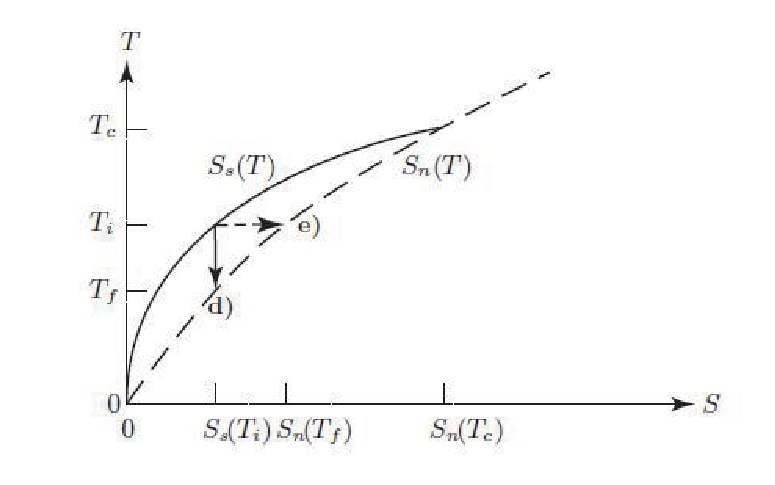
\includegraphics[scale=0.7]{chpt1/figs/fig1.7.eps}
  \caption{超导态(实线)和正常态(虚线)的T-S图}\label{fig:tsplot}
\end{figure}

e) 超导体被加热,首先必须先进入正常态。外场提供磁能$\mu_0 H_c^2(T_i)/2$;由于转变过程要吸热
$T_i[S_n(T-i)-S_s(T_i)]$,故还必须提供吸收能$H_{ec}$。图\ref{fig:tsplot}中的横虚线就是转变过程。于是,
\begin{align*}
\frac{1}{2}\mu_0 H_{ec}^2(T_i)=\frac{1}{2}\mu_0 H_c^2(T_i)+T_i[S_n(T_i)-S_s(T_i)]\tag{S1.21}
\end{align*}

上式和S1.1联立,得到
\begin{align*}
\frac{1}{2}\mu_0 H_{ec}^2(T_i)=\frac{1}{2}\mu_0 H_c^2(T_i)+T_i\left[\frac{1}{3}(b-a)T_i^3+\gamma T_i\right] \tag{S1.22}
\end{align*}

把S1.9代入上式,并应用S1.19,得到
\begin{align*}
frac{1}{2}\mu_0 H_{ec}^2(T_i)=\frac{1}{2}\mu_0 H_c^2(T_i)+2\mu_0 H_{c_0}^2\left(\frac{T_i}{T_c}\right)^2 \left[1-\left(\frac{T_i}{T_c}\right)^2 \right] \tag{S1.23}
\end{align*}

联立式\ref{eqn:1.7},得到
\begin{align*}
H_{ec}^2(T_i)=H_c^2(T_i)+4H_c^2(T_i)\frac{(T_i/T_c)^2}{1-(T_i/T_c)^2} \tag{S1.24}
\end{align*}

于是
\begin{align*}
H_{ec}(T_i)=H_c(T_i)\sqrt{\frac{1+3(T_i/T_c)^2}{1-(T_i/T_c)^2}}
\end{align*}

由于$H_c(T_c)=0$,可知$H_{ec}(T_c)=0$;另有$H_{ec}(T_i)\ge H_c(T_i)$。


\subsection{问题1.2:超导回路}
本问题表明,仅通过外接电源才能在闭合超导回路、线圈或盘中产生持续电流。
此处用电路模型证明,参数如图\ref{scloop}。
 
a) 写出两个回路的电路方程。

b) 解出$I_s(t)$,证明以一个初始态和末态都是0的$I(t)$($I(t=0)=I(t=\infty)=0$)不能建立起闭合回路的电流。
闭合超导回路可以是一个采用超导中间接头连接引线的超导磁体、超导盘片、超导盘片堆叠体、圆心有空的超导盘片或
圆心有孔的超导盘片堆叠体。

%图
\begin{figure}[htbp]
  \centering
 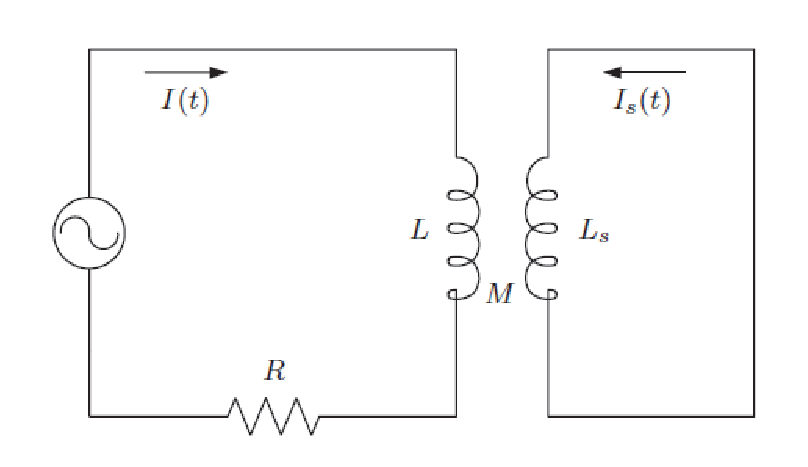
\includegraphics[scale=0.6]{chpt1/figs/fig1.8.eps}
  \caption{
超导线圈回路与一个带有电流源的回路通过电感耦合
}\label{scloop}
\end{figure}

\subsubsection{问题1.2之解答}
a) 两个电压方程为
\begin{align*}
L\frac{dI(t)}{dt}+M\frac{dI_s(t)}{dt}+ RI(t) = 0 \tag{S2.1a}
\end{align*}
\begin{align*}
M\frac{dI(t)}{dt}+ L_s\frac{dI_s(t)}{dt}= 0 \tag{S2.1b}
\end{align*}

b) 从S2.1b中可以解得
\begin{align*}
I_s(t) = −\frac{M}{L_s}I(t) + C\tag{S2.2}
\end{align*}

因为$I_s(t=0)=0$,所以,$C=0$。由于$I(t=0)=I(t=\infty)=0$,所以仅在$I(t)\neq 0$时有$I_s(t)\neq 0$。
也即,无外流源也无初始值的超导回路不能孤立的维持能量。

在一个超导回路中不能产生感应电流在某些应用中是有实际意义的。持续运行模式的磁体必须通过引线通入电流
充电(处于励磁模式)。此后,通过所谓的``超导开关"(persistent current switch,PCS)将引线短路后电源可以退出。


\subsection{问题1.3:磁共振成像(MRI)}
超导磁体最成功的商业应用之一便是医疗诊断装置,特别是MRI。以下是磁体工程师需要了解的一些基本问题:

a) MRI中,为什么$H^1$、$N^{14}$核可以被探测到,而$C^{12}$、$O^{16}$核探测不到?

b) 如果频率分辨率10 Hz,对于1 T全身MRI磁体的中心磁场均匀性最小要求多少?对室温孔直径80 cm的全身MRI磁体,
上述均匀场区域通常在25 cm DSU(直径半球体积)。

c) MRI单元中,脉冲梯度磁体的作用?

d) 对1 T磁体单元,脉冲磁体产生的典型$\frac{d\vec{B}}{dz}$是多少?

\subsubsection{问题1.3之解答}
a) 有奇数核子的原子核存在净角动量。处于磁场中,原子核按某种正比于磁场强度的特定频率(Larmor)进动。
比如氢的Larmor频率在1 T时是42.576 MHz。表1.6\footnote{加粗的数字表示可探测}给出了几种物质原子的数据。
%表1.6
\begin{table}[htbp]\small
  \centering
  \caption{几种元素的原子核数据} \label{tb:atomic}
\begin{tabular}{|c|c|c|c|c|c|}
  \hline
原子序数&元素&原子质量&质子数&中子数&可探测? \\ \hline \hline
1&氢&1&\textbf{1}&0&是 \\ \hline
6&碳&12&6&6&否 \\ \hline
6&碳&13&6&\textbf{7}&是 \\ \hline
7&氮&14&\textbf{7}&\textbf{7}&是 \\ \hline
8&氧&16&8&8&否 \\ \hline
11&钠&23&\textbf{11}&12&是 \\ \hline
15&磷&31&\textbf{15}&16&是 \\ \hline
\end{tabular}
\end{table}

b) 10 Hz相当于 $42.576×10^6$ Hz的$0.23×10^{−6}$,所以磁场必须是1 T的$0.23×10^{−6}$ ,
大约是 $0.002\ \mathrm{gauss}$。作为对比,地磁场约为$0.7 \ \mathrm{gauss}$。

c) 通过引入特定的空间磁场分布,我们可以限制在某个指定区域产生共振。
这让我们可以对某一个特定核素进行成像。

d) 梯度幅值直接和成像的空间解析度相关。更高的梯度相应产生更好的解析度。但存在一个磁体
和患者可以忍受的极限问题。医用MRI必须限制梯度强度---至少应限制梯度偏斜率---以避免产生对神经
和肌肉的刺激。医用MRI的最大梯度约为$3-4 \ \mathrm{gauss/cm}$,最大场偏斜率约为$12\ \mathrm{(gauss/cm)/ms}$或者
$120\ \mathrm{(T/m)/s}$。

\section*{参考文献}
[1.1] J.K. Hulm and B.T. Matthias, “Overview of superconducting materials development,”
in Superconductor Materials Science—Metallurgy, Fabrication, and Applications,
Eds., S. Foner and B.B. Schwartz (Plenum Press, NewYork, 1981).

[1.2] A.A. Abrikosov, “On the magnetic properties of superconductors of the second
type (English translation),” Zh. Eksp. Teor. Fiz. (Soviet Union) 5, 1174 (1957).

[1.3] U. Essmann and H. Tr¨auble, “The direct observation of individual flux lines in
Type II superconductors,” Phys. Lett. 24A, 526 (1967).

[1.4] Y.B. Kim, C.F. Hempstead, and A.R. Strnad, “Magnetization and critical supercurrents,” Phys. Rev. 129, 528 (1963).

[1.5] J.K. Hoffer, “The Initiation and propagation of normal zones in a force-cooled
tubular superconductor,” IEEE Trans. Mag. 15, 331 (1979).

[1.6] C. Marinucci, M.A. Hilal, J. Zellweger, and G. Vecsey, “Quench studies of the
Swiss LCT conductor,” Proc. 8th Symp. on Eng. Prob. Fus. Res., 1424 (1979).

[1.7] V.D. Arp, “Stability and thermal quenches in force-cooled superconducting cables,”
Proc. of 1980 Superconducting MHD Magnet Design Conference, MIT, 142(1980).

[1.8] J. Benkowitsch and G. Kraft, “Numerical analysis of heat-induced transients in
forced flow helium cooling systems,” Cryogenics 20, 209 (1980).

[1.9] E.A. Ibrahim, “Thermohydraulic Analysis of Internally Cooled Superconductors,”
Adv. Cryo. Eng. 27, 235 (1982).

[1.10] C. Marinucci, “A numerical model for the analysis of stability and quench characteristics of forced-flow cooled superconductors,” Cryogenics 23, 579 (1983).

[1.11] M.C.M. Cornellissen and C.J. Hoogendoorn, “Propagation velocity for a force
cooled superconductor,” Cryogenics 25, 185 (1985).

[1.12] A.F. Volkov, L.B. Dinaburg, and V.V. Kalinin, “Simulation of helium pressure
rise in hollow conductor in case of superconductivity loss,” Proc. 12th Int. Cryo.
Eng. Conf. (Southampton, UK), 922 (1988).

[1.13] R.L. Wong, “Program CICC flow and heat transfer in cable-in-conduit conductors,”
Proc. 13th Symp. Fus. Tech. (Knoxville, TN), 1134 (1989).

[1.14] L. Bottura and O.C. Zienkiewicz, “Quench analysis of large superconducting magnets. Part I: model description,” Cryogenics 32, 659 (1992).

[1.15] C.A. Luongo, C.-L. Chang, and K.D. Partain, “A computational model applicable
to the SMES/CICC,” IEEE Trans. Mag. 30, 2569 (1994).

[1.16] A. Shajii and J.P. Freidberg, “Quench in superconducting magnets. I. Model and
implementation,” J. Appl. Phys. 76, 3149 (1994); “Quench in superconducting
magnets. II. Analytic Solution,” J. Appl. Phys. 76, 3159 (1994).

[1.17] R. Zanino, S. De Palo, and L. Bottura, “A two-fluid code for the thermohydraulic
transient analysis of CICC superconducting magnets,” J. Fus. Energy 14,
25 (1995).

[1.18] L. Bottura, “A numerical model for the simulation of quench in the ITER magnets,”
J. Comp. Phys. 125, 26 (1996).

[1.19] L Bottura, C. Rosso, and M. Breschi, “A general model for thermal, hydraulic,
and electric analysis of superconducting cables,” Cryogenics 40, 617 (2000).

[1.20] Q. Wang, P. Weng, and M. Hec, “Simulation of quench for the cable-in-conduitconductor in HT-7U superconducting Tokamak magnets using porous medium
model,” Cryogenics 44, 81 (2004).

[1.21] T. Inaguchi, M. Hasegawa, N. Koizumi, T. Isono, K. Hamada, M. Sugimoto, and
Y. Takahashi, “Quench analysis of an ITER 13T-40kA Nb3Sn coil (CS insert),”
Cryogenics 44, 121 (2004).

[1.22] L. Bottura, “Numerical aspects in the simulation of thermohydraulic transients
in CICC’s,” J. Fus. Energy 14, 13 (1995).

[1.23] L. Bottura and A. Shajii, “Numerical quenchback in thermofluid simulations of
superconducting magnets,” Int. J. Num. Methods Eng. 43, 1275 (1998).

[1.24] L. Bottura, “Modelling stability in superconducting cables,” Physica C 316 (1998).

[1.25] A.B. Pippard, The Elements of Classical Thermodynamics (Cambridge University
Press, Cambridge, 1966).

[1.26] C. Kittel, Introduction to Solid State Physics 3rd Ed. (John Wiley \& Sons, 1966).
